\documentclass[11pt]{article}
\usepackage{graphicx}
\pagestyle{myheadings}

% -----------------------------------------------------------------------------
% ? Document identification
\newcommand{\stardoccategory}  {Starlink User Note}
\newcommand{\stardocinitials}  {SUN}
\newcommand{\stardocsource}    {sun\stardocnumber}
\newcommand{\stardocnumber}    {146.4}
\newcommand{\stardocauthors}   {Julian Osborne, Jeremy Ashley, \& Grant Privett}
\newcommand{\stardocdate}      {25th June 1996}
\newcommand{\stardoctitle}     {OBSERVE --- Check Star Observability}
\newcommand{\stardocversion}   {Version 2.2}
\newcommand{\stardocmanual}    {User's Guide}
\newcommand{\stardocabstract}  {[Text of abstract]}
% ? End of document identification

% -----------------------------------------------------------------------------

\newcommand{\stardocname}{\stardocinitials /\stardocnumber}
\markright{\stardocname}
\setlength{\textwidth}{160mm}
\setlength{\textheight}{230mm}
\setlength{\topmargin}{-2mm}
\setlength{\oddsidemargin}{0mm}
\setlength{\evensidemargin}{0mm}
\setlength{\parindent}{0mm}
\setlength{\parskip}{\medskipamount}
\setlength{\unitlength}{1mm}

% -----------------------------------------------------------------------------
%  Hypertext definitions.
%  ======================
%  These are used by the LaTeX2HTML translator in conjunction with star2html.

%  Comment.sty: Version 2.0, 19 June 1992
%  Selectively in/exclude pieces of text.
%
%  Author
%    Victor Eijkhout                                      <eijkhout@cs.utk.edu>
%    Department of Computer Science
%    University Tennessee at Knoxville
%    104 Ayres Hall
%    Knoxville, TN 37996
%    USA

%  Do not remove the %begin{latexonly} and %end{latexonly} lines (used by
%  star2html to signify raw TeX that latex2html cannot process).
%begin{latexonly}
\makeatletter
\def\makeinnocent#1{\catcode`#1=12 }
\def\csarg#1#2{\expandafter#1\csname#2\endcsname}

\def\ThrowAwayComment#1{\begingroup
    \def\CurrentComment{#1}%
    \let\do\makeinnocent \dospecials
    \makeinnocent\^^L% and whatever other special cases
    \endlinechar`\^^M \catcode`\^^M=12 \xComment}
{\catcode`\^^M=12 \endlinechar=-1 %
 \gdef\xComment#1^^M{\def\test{#1}
      \csarg\ifx{PlainEnd\CurrentComment Test}\test
          \let\html@next\endgroup
      \else \csarg\ifx{LaLaEnd\CurrentComment Test}\test
            \edef\html@next{\endgroup\noexpand\end{\CurrentComment}}
      \else \let\html@next\xComment
      \fi \fi \html@next}
}
\makeatother

\def\includecomment
 #1{\expandafter\def\csname#1\endcsname{}%
    \expandafter\def\csname end#1\endcsname{}}
\def\excludecomment
 #1{\expandafter\def\csname#1\endcsname{\ThrowAwayComment{#1}}%
    {\escapechar=-1\relax
     \csarg\xdef{PlainEnd#1Test}{\string\\end#1}%
     \csarg\xdef{LaLaEnd#1Test}{\string\\end\string\{#1\string\}}%
    }}

%  Define environments that ignore their contents.
\excludecomment{comment}
\excludecomment{rawhtml}
\excludecomment{htmlonly}

%  Hypertext commands etc. This is a condensed version of the html.sty
%  file supplied with LaTeX2HTML by: Nikos Drakos <nikos@cbl.leeds.ac.uk> &
%  Jelle van Zeijl <jvzeijl@isou17.estec.esa.nl>. The LaTeX2HTML documentation
%  should be consulted about all commands (and the environments defined above)
%  except \xref and \xlabel which are Starlink specific.

\newcommand{\htmladdnormallinkfoot}[2]{#1\footnote{#2}}
\newcommand{\htmladdnormallink}[2]{#1}
\newcommand{\htmladdimg}[1]{}
\newenvironment{latexonly}{}{}
\newcommand{\hyperref}[4]{#2\ref{#4}#3}
\newcommand{\htmlref}[2]{#1}
\newcommand{\htmlimage}[1]{}
\newcommand{\htmladdtonavigation}[1]{}
\newcommand{\latexhtml}[2]{#1}
\newcommand{\html}[1]{}

%  Starlink cross-references and labels.
\newcommand{\xref}[3]{#1}
\newcommand{\xlabel}[1]{}

%  LaTeX2HTML symbol.
\newcommand{\latextohtml}{{\bf LaTeX}{2}{\tt{HTML}}}

%  Define command to re-centre underscore for Latex and leave as normal
%  for HTML (severe problems with \_ in tabbing environments and \_\_
%  generally otherwise).
\newcommand{\latex}[1]{#1}
\newcommand{\setunderscore}{\renewcommand{\_}{{\tt\symbol{95}}}}
\latex{\setunderscore}

%  Redefine the \tableofcontents command. This procrastination is necessary
%  to stop the automatic creation of a second table of contents page
%  by latex2html.
\newcommand{\latexonlytoc}[0]{\tableofcontents}

% -----------------------------------------------------------------------------
%  Debugging.
%  =========
%  Remove % on the following to debug links in the HTML version using Latex.

% \newcommand{\hotlink}[2]{\fbox{\begin{tabular}[t]{@{}c@{}}#1\\\hline{\footnotesize #2}\end{tabular}}}
% \renewcommand{\htmladdnormallinkfoot}[2]{\hotlink{#1}{#2}}
% \renewcommand{\htmladdnormallink}[2]{\hotlink{#1}{#2}}
% \renewcommand{\hyperref}[4]{\hotlink{#1}{\S\ref{#4}}}
% \renewcommand{\htmlref}[2]{\hotlink{#1}{\S\ref{#2}}}
% \renewcommand{\xref}[3]{\hotlink{#1}{#2 -- #3}}
%end{latexonly}
% -----------------------------------------------------------------------------
% ? Document specific \newcommand or \newenvironment commands.

% Environment for indenting and using a small font.
\newenvironment{myquote}{\begin{quote}\begin{small}}{\end{small}\end{quote}}

% in-line verbatims
\newcommand{\myverb}[1]{{\small \verb+#1+}}

% degrees symbol - requires hypertext to be post processed.
\newcommand{\degrees}{\hbox{$^\circ$}}
\begin{htmlonly}
\newcommand{\degrees}{{\rawhtml &deg;}}
\end{htmlonly}

% ? End of document specific commands
% -----------------------------------------------------------------------------
%  Title Page.
%  ===========
% \renewcommand{\thepage}{\roman{page}}
\begin{document}
\thispagestyle{empty}

%  Latex document header.
%  ======================
\begin{latexonly}
   CCLRC / {\sc Rutherford Appleton Laboratory} \hfill {\bf \stardocname}\\
   {\large Particle Physics \& Astronomy Research Council}\\
   {\large Starlink Project\\}
   {\large \stardoccategory\ \stardocnumber}
   \begin{flushright}
   \stardocauthors\\
   \stardocdate
   \end{flushright}
   \vspace{-4mm}
   \rule{\textwidth}{0.5mm}
   \vspace{5mm}
   \begin{center}
   {\Huge\bf  \stardoctitle \\ [2.5ex]}
   {\LARGE\bf \stardocversion \\ [4ex]}
   {\Huge\bf  \stardocmanual}
   \end{center}
   \vspace{5mm}

% ? Heading for abstract if used.
%  \vspace{10mm}
%  \begin{center}
%     {\Large\bf Abstract}
%  \end{center}
% ? End of heading for abstract.
\end{latexonly}

%  HTML documentation header.
%  ==========================
\begin{htmlonly}
   \xlabel{}
   \begin{rawhtml} <H1> \end{rawhtml}
      \stardoctitle\\
      \stardocversion\\
      \stardocmanual
   \begin{rawhtml} </H1> \end{rawhtml}

% ? Add picture here if required.
% ? End of picture

   \begin{rawhtml} <P> <I> \end{rawhtml}
   \stardoccategory\ \stardocnumber \\
   \stardocauthors \\
   \stardocdate
   \begin{rawhtml} </I> </P> <H3> \end{rawhtml}
      \htmladdnormallink{CCLRC}{http://www.cclrc.ac.uk} /
      \htmladdnormallink{Rutherford Appleton Laboratory}
                        {http://www.cclrc.ac.uk/ral} \\
      \htmladdnormallink{Particle Physics \& Astronomy Research Council}
                        {http://www.pparc.ac.uk} \\
   \begin{rawhtml} </H3> <H2> \end{rawhtml}
      \htmladdnormallink{Starlink Project}{http://www.starlink.ac.uk/}
   \begin{rawhtml} </H2> \end{rawhtml}
   \htmladdnormallink{\htmladdimg{source.gif} Retrieve hardcopy}
      {http://www.starlink.ac.uk/cgi-bin/hcserver?\stardocsource}\\

%  HTML document table of contents.
%  ================================
%  Add table of contents header and a navigation button to return to this
%  point in the document (this should always go before the abstract \section).
  \label{stardoccontents}
  \begin{rawhtml}
    <HR>
    <H2>Contents</H2>
  \end{rawhtml}
  \renewcommand{\latexonlytoc}[0]{}
  \htmladdtonavigation{\htmlref{\htmladdimg{contents_motif.gif}}
        {stardoccontents}}

% ? New section for abstract if used.
% \section{\xlabel{abstract}Abstract}
% ? End of new section for abstract
\end{htmlonly}

% -----------------------------------------------------------------------------
% ? Document Abstract. (if used)
%  ==================
% \stardocabstract
% ? End of document abstract
% -----------------------------------------------------------------------------
% ? Latex document Table of Contents (if used).
%  ===========================================
%  \newpage
 \begin{latexonly}
   \setlength{\parskip}{0mm}
   \latexonlytoc
   \setlength{\parskip}{\medskipamount}
   \markright{\stardocname}
 \end{latexonly}
% ? End of Latex document table of contents
% -----------------------------------------------------------------------------
\newpage
% \renewcommand{\thepage}{\arabic{page}}
% \setcounter{page}{1}

\section{\xlabel{VERSION}This Version}
\label{sec:version}

This document refers to \stardocversion\ of the programme {\bf{observe}}.
This third release of the programme will run on a variety of UNIX
computers.

A number of changes have been made in {\bf{observe}} \stardocversion.
It now makes use of the ADAM parameter system and does not employ
routines from {\sc ASTERIX} for printing information to the screen. It
also presents the user with the full list of telescopes from SLALIB,
allowing a wider choice of pre-defined observing sites.

In addition, much of the information displayed in graphical format
can now be output to a simple text file.

Our thanks go to a number of users for suggesting these changes.

\section{\xlabel{INTRODUCTION}Introduction}
\label{sec:introduction}

The programme {\bf{observe}} is designed to allow you to get a quick
overview of the observability of a star through the year from the
geographical location selected. You will be prompted for the RA and Dec
of the star, the telescope (you can also specify arbitrary locations),
and the year. On the selected GKS graphics device a plot will be drawn
that tells you, for all dates of the year, the star rising and setting
times and the times that it is 30\degrees\ above the  horizon, the
times of astronomical twilight, the phase and rising and setting  times
of the Moon as well as its distance from the star in question.

The algorithms used in calculating these times, positions and phases
come from the book {\em{`Practical Astronomy with your calculator'}}  by
P.\,Duffett-Smith (3$^{\rm rd}$ ed.~CUP 1988), and are used with
permission. These algorithms are not designed for high-precision
calculations, a fact which is to some extent conveyed by the programme
output. Nevertheless, we have verified that the routines are good for
their purpose.

As mentioned above, all standard Starlink graphics devices are
supported.  However, the graphical output created by {\bf{observe}} is
sufficiently complicated and the device drivers have sufficiently
different effects that plotting to a laser printer is almost certainly
the best option. We recommend that the GKS landscape postscript device
{\tt{ps\_l}} is chosen.  The following command will then print the
output file ({\tt{\%}} is the shell prompt):

\begin{verbatim}
      % lpr -Pstar_post gks74.ps
\end{verbatim}

where {\tt{star\_post}} is the name of the postscript printer.
(Subsequent plots to this device produce filenames {\tt gks74.ps.1},
{\em{etc}}). You can also look at this output file on an X-terminal
using {\bf{ghostview}} in landscape mode.

The programme {\bf{observe}} was originally created by Manfred Gottwald,
then of the EXOSAT Observatory. We have increased the quantity of
information displayed and increased the list of standard observatories,
and now take responsibility for this software.


\section{\xlabel{DESCRIPTION}Description of the Output}
\label{sec:description}

One screen of graphics is drawn per star. This consists of a header, a
large plot, and some lines of text explanation. The plot is formatted
with date through the year shown horizontally and time through the day
shown vertically. The  left-hand scale shows UT and the right-hand
scale shows local time with midnight at the centre. Figure
\ref{fig:sum} shows a summary of the symbols used in the plot.

\begin{figure}[h]\caption{Summary of OBSERVE Plot Symbols}
\label{fig:sum}
\begin{center}
\begin{tabular}{|c|l|}
\hline
\large
---{\sf X}--- & start of astronomical night \\
---{\sf V}--- & end of astronomical night \\
---$\uparrow$--- & star rises \\
---$\downarrow$--- & star sets \\
---$\circ$--- & star rises above 30$^o$ elevation\\
---$\bullet$--- & star falls below 30$^o$ elevation\\
- - - - & great circle Moon-star distance \\
\rule{0.1mm}{4mm} & 25\%--50\% illuminated Moon above horizon\\
\rule{0.3mm}{4mm} & 50\%--75\% illuminated Moon above horizon\\
\rule{0.5mm}{4mm} & 75\%--100\% illuminated Moon above horizon\\
\hline
\end{tabular}
\end{center}
\end{figure}

\subsection{The start and end of the night}

Wavy horizontal solid lines show the start and end of the  astronomical
night.  Symbol {\sf{X}}  shows the start of the night ({\em{i.e.}},~the
end of day-to-night astronomical  twilight), and  symbol {\sf{V}} shows
the end of the night ({\em{i.e.}},~the start of night-to-day
astronomical twilight). For extreme  northerly and southerly
geographical locations these lines merge to become a closed shape as
there is no astronomical night during polar summer.

\subsection{The rising and setting of the star}

Straight diagonal solid lines marked with symbols  show the times of
star rising ($\uparrow$) and setting ($\downarrow$). Parallel lines
show the times at  which the star rises above ($\circ$) and sets below
($\bullet$) 30\degrees\ elevation, a typical minimum elevation for
useful observing.

\subsection{The Moon}

The remaining lines in the plot refer to the Moon. The great-circle
distance of the Moon from the star is shown (in hours) by a dashed
sinewave in the top half of the plot. Read the distance off the
right-hand scale and multiply by 15 to get the distance in degrees.

The rising and setting of the Moon is shown by vertical solid lines of
variable width.  A line is plotted for every other day, it starts at
the time of moonrise and ends at the time of moonset.  The width of the
Moon lines are related to the phase of  the Moon for that date. The
thickest lines are plotted when the Moon is  75\%-100\% illuminated,
thinner lines are plotted for 50\%-75\% and 25\%-50\% illumination. No
line is plotted when the fractional illumination is less than  25\%.

\subsection{How to look at the plot}

The region of visibility of the star typically falls halfway down the
plot (between the wavy lines), and is bounded on left and right by
diagonal lines with empty and filled  circles superimposed. Depending
on the nature of the observation planned, you may then need  to look
for  dates and/or times clear of the vertical Moon lines.

\subsection{Text file Output}

If you reply 'yes' to the {\tt{TEXTF}} parameter, {\bf{observe}} will
create a text file that contains the star rise and set times, the times
at which the star rises above or moves below 30\degrees\ above the
horizon, the times when astronomical twilight begins and end, the
distance star/Moon separation and the moon phase for every day of the
year chosen.

\newpage
\section{An Example}

Suppose that you want to check when the bright star Mira can be
observed  from the AAT.  You should enter the command {\bf{observe}} and
respond to the questions as  shown:

\begin{quote}\small
\begin{verbatim}
> observe
OBSERVE V2.2

  1) Anglo-Australian 3.9m  2) William Herschel 4.2m  3) Isaac Newton 2.5m Tel
  4) Jacobus Kapteyn 1m Te  5) Lick 120 inch          6) MMT, Mt Hopkins
  7) DAO Victoria BC 1.85   8) Du Pont 2.5m Telescop  9) Mt Hopkins 1.5 metre
 10) Mount Stromlo 74 inch 11) Siding Spring 2.3 met 12) Greenbank 140 foot
 13) Cerro Tololo 4 metre  14) Cerro Tololo 1.5 metr 15) Tidbinbilla 64 metre
 16) Bloemfontein 1.52 met 17) Bosque Alegre 1.54 me 18) USNO 61 inch astrogra
 19) Perkins 72 inch, Lowe 20) Harvard College Obser 21) Okayama 1.88 metre
 22) Kitt Peak 158 inch    23) Kitt Peak 90 inch     24) Kitt Peak 84 inch
 25) Kitt Peak 36 foot     26) Kottamia 74 inch      27) ESO 3.6 metre
 28) Mauna Kea 88 inch     29) UK Infra Red Telescop 30) Quebec 1.6 metre
 31) Mt Ekar 1.82 metre    32) Mt Lemmon 60 inch     33) McDonald 2.7 metre
 34) McDonald 2.1 metre    35) Palomar 200 inch      36) Palomar 60 inch
 37) David Dunlap 74 inch  38) Haute Provence 1.93 m 39) Haute Provence 1.52 m
 40) San Pedro Martir 83 i 41) Sutherland 74 inch    42) Tautenburg 2 metre
 43) Catalina 61 inch      44) Steward 90 inch       45) USSR 6 metre
 46) Arecibo 1000 foot     47) Cambridge 5km         48) Cambridge 1 mile
 49) Effelsberg 100 metre  50) Greenbank 300 foot    51) Jodrell Bank 250 foot
 52) Parkes 64 metre       53) Very Large Array      54) Sugar Grove 150 foot
 55) USSR 600 foot         56) Nobeyama 45 metre     57) JCMT 15 metre
 58) ESO 3.5 metre NTT     59) St Andrews            60) Apache Point 3.5m
 61) Keck 10m Telescope #1 62) Tautenberg 1.34 metre 63) Palomar 48-inch Schmi
 64) UK 1.2 metre Schmidt, 65) Kiso 1.05 metre Schmi 66) ESO 1 metre Schmidt,
 67) Australia Telescope C

NUMBER - Enter telescope number, or 0 for other /1/ >
STAR - Name of object /'Mira'/ >
RA - Object coordinates (hh mm ss) /'02 16 48.'/ >
DEC - Object coordinates (dd mm ss) /'-3 12 0'/ >
YEAR - Year of observation /1994/ >
Calculating rise times etc.
DEVICE - Output graphics device (e.g. ps_l) /'ps_l'/ >
Plotting Visibility graph.
TEXTF - Want text file output? /TRUE/ >
OUT - Text file name /@0/ > outputfile
AGAIN - New telescope (T); New Star (S); Both (B) or QUIT (Q) > q
>
> lpr -Pstar_post gks74.ps
\end{verbatim}
\end{quote}

Figure~\ref{fig_output} shows the result of the above query.
From the description of the graph in section~\ref{sec:description},
you can see in this example that Mira is observable almost all year
from the AAT.  The longest observations are possible between
mid-January to mid-May, because  between these dates daylight does not
intrude when the star is above 30\degrees\ elevation. Good dates for
getting a long observation would be early February, April or May
because the Moon is close to new, although it is quite close to Mira
then.  For example, around February 11 1994 Mira would be visible from
the AAT between 14:00 UT and 21:40 UT, {\em{i.e.}},~midnight to 07:40
local time.

\newpage

\begin{figure}
\begin{center}
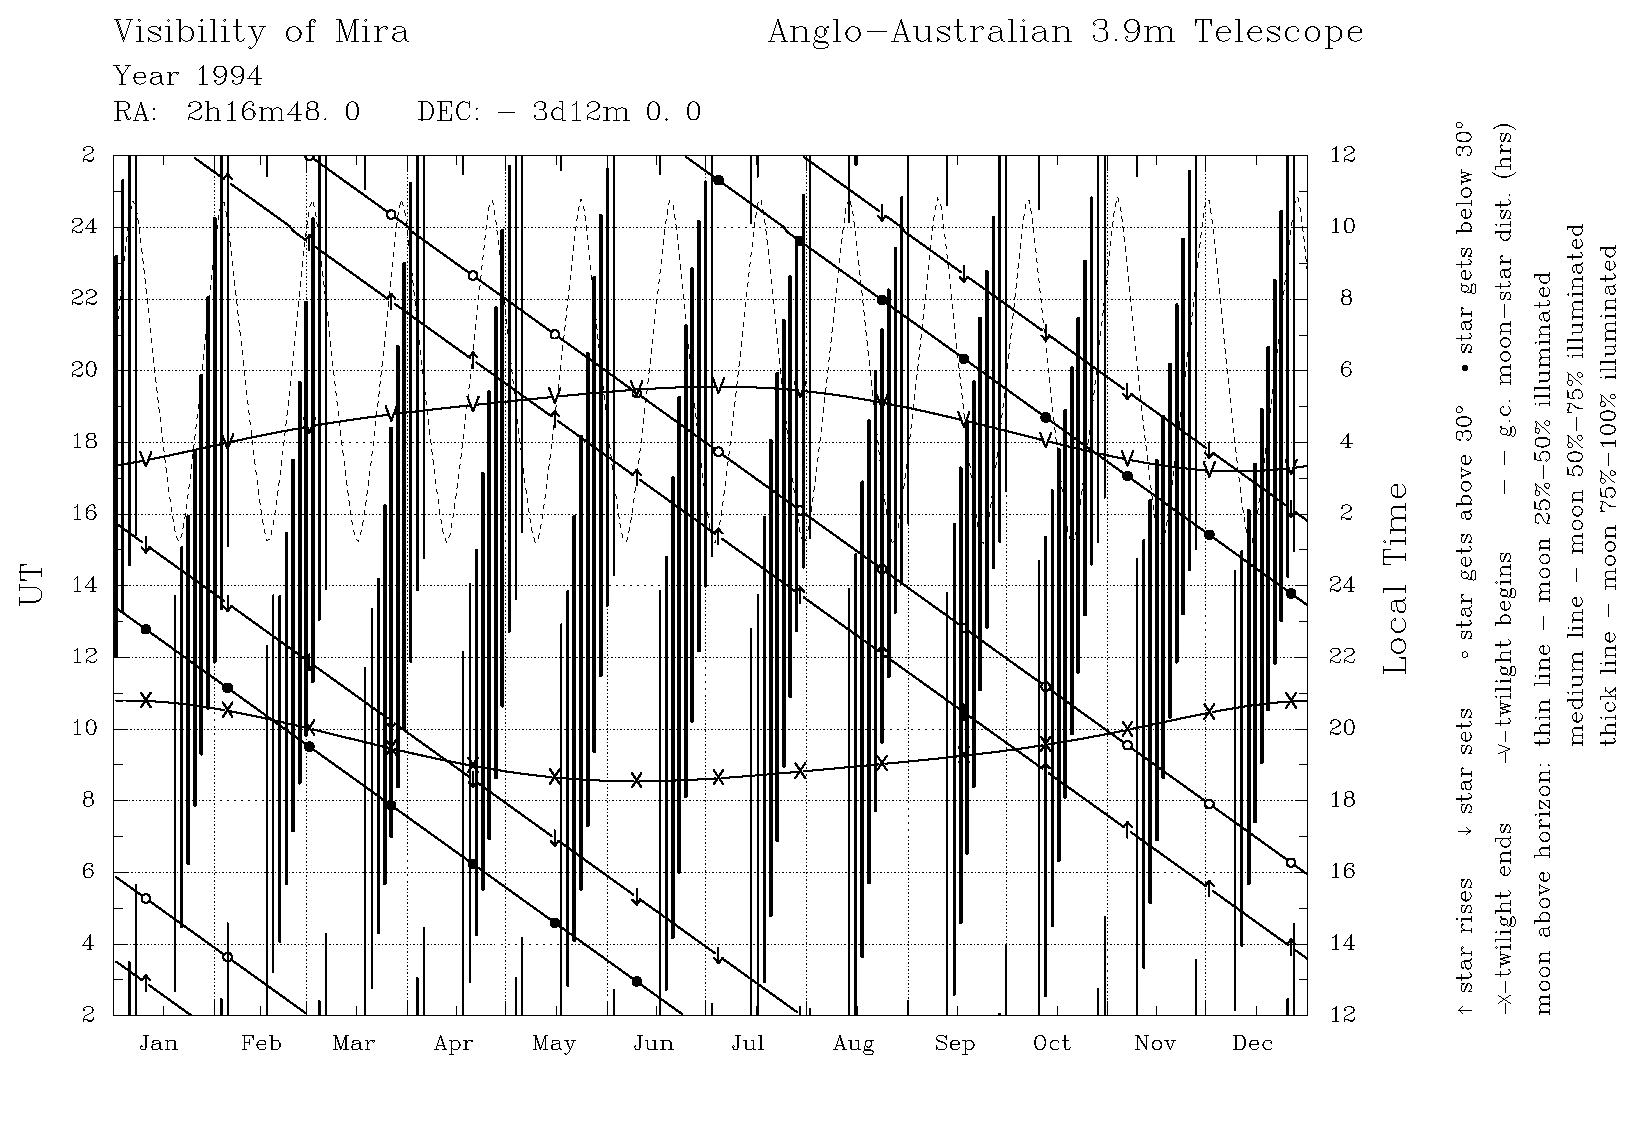
\includegraphics[angle=-180,width=\textwidth]{sun146_fig}
\vspace{5mm}
\caption{Graphic output from {\bf{observe}}.}
\label{fig_output}
\xlabel{fig_output}
\end{center}
\end{figure}

\end{document}
